\section{设计思想}
% 本程序中用到的所有数据类型的定义,主程序的流程图及各程序模块之间的调用关系
\subsection{逻辑设计}
\subsubsection{二叉树}
\paragraph{整体设计}作为一个数据结构,我希望它是泛型的,所以在实现二叉树的时候进行了泛型的支持。很多时候我们需要去访问各个节点的数据,因此这里提供了接口用于对节点进行操作,实现的默认方法是对数据进行打印,在这一部分使用了一些C++11的高级特性,比如lambda和function。为了可以直观的表示图的结构,我采用了输出dot图的方式,并使用了前面提到的访问接口,尽量重用了代码。便于对树的节点能有更高的自由度,实现了一个简易的迭代器,可以方便的进行节点的单步操作。

\paragraph{节点}二叉树的节点设计如下:

\begin{lstlisting}[language = c++]
    struct BitNode {
    // 约定lTag为true时,left或right是有效值
    Comparable data;
    bool lTag;
    bool rTag;
    BitNode *left;
    BitNode *right;
    };
\end{lstlisting}

\paragraph{迭代器}可使用不同模式对树进行遍历(建立在线索化的基础上)。

\begin{lstlisting}[language = c++]
    class Iterator {
    public:
    Iterator(BitNode *Root, Mode theMode) : header(Root), mode(theMode), isEnd(header == nullptr);
    const BitNode *operator*();
    void operator++(int);
    const bool &IsEnd();
    private:
    const BitNodePtr header;
    Mode mode;
    const BitNode *curr;
    bool isEnd;
    void preNext();
    void inNext();
    void postNext();
    const BitNode *findFather(const BitNode *child);
    }
\end{lstlisting}

\subsubsection{整体依赖关系图}

\begin{figure}[H]
    \centering
    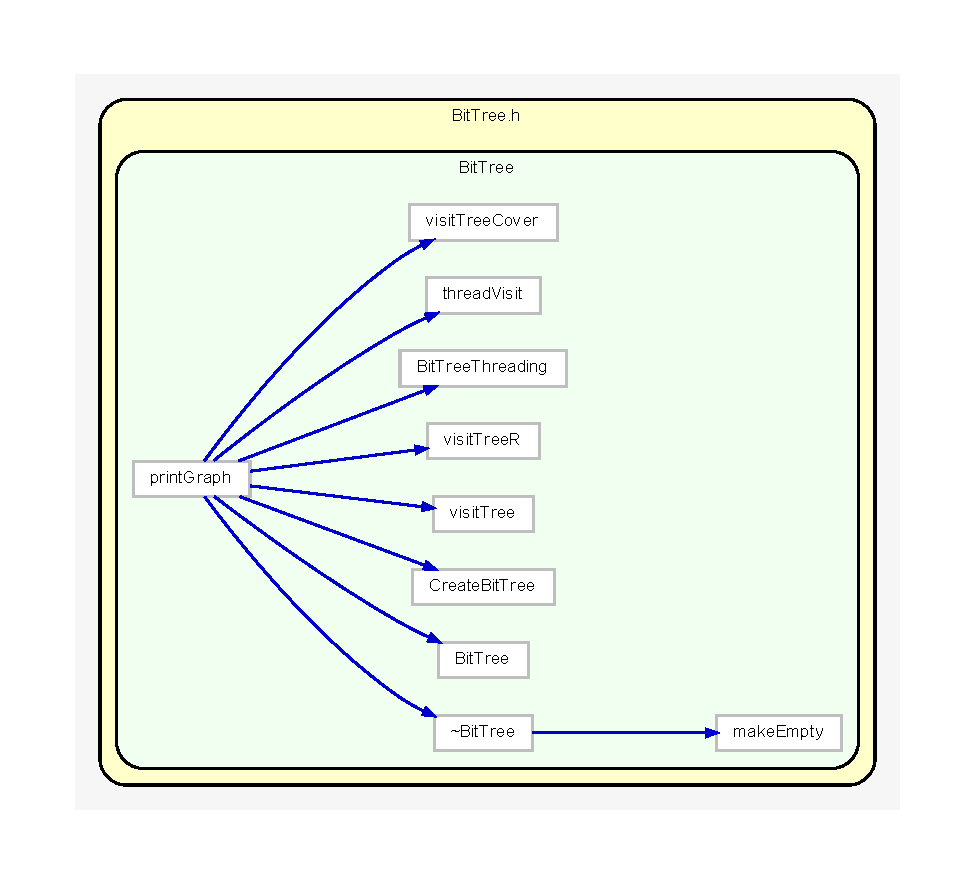
\includegraphics[width=0.7\linewidth]{figures/BitTree}
    \caption{整体依赖关系图}
    \label{fig:bittree}
\end{figure}


\subsection{Main函数流程图}
\begin{tikzpicture}
    \def \smbwd{2cm}
    \thispagestyle{empty}

    %定义流程图的具体形状
    \node (start) at (0,0) [draw, terminal,minimum width=\smbwd, minimum height=0.5cm] {开始}; % 定义开始
    \node (getdata) at (0,-1) [draw, predproc, align=left,minimum width=\smbwd,minimum height=0.5cm] {从文件或者预定义部分读取数据};
    \node (makeTree) at (0,-2) [draw, storage, minimum width=\smbwd, minimum height=0.5cm] {构建二叉树};
    \node (out) at (0,-3) [draw, process, minimum width=\smbwd, minimum height=0.5cm] {非递归输出二叉树数据};
    \node (outR) at (0,-4) [draw, process, minimum width=\smbwd, minimum height=0.5cm] {递归输出二叉树数据};
    \node (makeThread) at (0,-5) [draw, storage, minimum width=\smbwd, minimum height=0.5cm] {线索化二叉树};
    \node (printTree) at (0,-6) [draw, process, minimum width=\smbwd, minimum height=0.5cm] {绘制线索二叉树};
    \node (outThread) at (0,-7) [draw, storage, minimum width=\smbwd, minimum height=0.5cm] {线索输出二叉树};
    \node (end) at (0,-8) [draw, terminal,minimum width=\smbwd,minimum height=0.5cm] {结束}; %定义结束

    %连接定义的形状,绘制流程图--表示垂直线,|表示箭头方向
    \draw[-] (start) -- (getdata) -- (makeTree) -- (out) -- (outR) -- (makeThread) -- (printTree) -- (outThread) -- (end);

\end{tikzpicture}